\documentclass[onecolumn, draftclsnofoot,10pt, compsoc]{IEEEtran}
\usepackage{graphicx}
\usepackage{url}
\usepackage{setspace}
\usepackage[final]{pdfpages}

\usepackage{geometry}
\geometry{textheight=9.5in, textwidth=7in}

% 1. Fill in these details
\def \CapstoneTeamName{		Malsano}
\def \CapstoneTeamNumber{		72}
\def \GroupMemberOne{			Brandon Jolly}
\def \GroupMemberTwo{			Katherine Jeffrey}
\def \GroupMemberThree{			Bradford Wong}
\def \CapstoneProjectName{		App to Support Field Diagnostics in Veterinary Medicine}
\def \CapstoneSponsorCompany{	Oregon Veterinary Diagnostic Laboratory}
\def \CapstoneSponsorPerson{		Dr. Christiane Loehr}

% 2. Uncomment the appropriate line below so that the document type works
\def \DocType{		%Problem Statement
				Weekly Blog Reports(Bradford Wong)
				%Technology Review
				%Design Document
				%Progress Report
				}
			
\newcommand{\NameSigPair}[1]{\par
\makebox[2.75in][r]{#1} \hfil 	\makebox[3.25in]{\makebox[2.25in]{\hrulefill} \hfill		\makebox[.75in]{\hrulefill}}
\par\vspace{-12pt} \textit{\tiny\noindent
\makebox[2.75in]{} \hfil		\makebox[3.25in]{\makebox[2.25in][r]{Signature} \hfill	\makebox[.75in][r]{Date}}}}
%3. If the document is not to be signed, uncomment the RENEWcommand below
%\renewcommand{\NameSigPair}[1]{#1}

%%%%%%%%%%%%%%%%%%%%%%%%%%%%%%%%%%%%%%%
\begin{document}
\begin{titlepage}
    \pagenumbering{gobble}
    \begin{singlespace}
%    	
\includegraphics[height=4cm]{coe_v_spot1}
        \hfill 
        % 4. If you have a logo, use this includegraphics command to put it on the coversheet.
        %\includegraphics[height=4cm]{CompanyLogo}   
        \par\vspace{.2in}
        \centering
        \scshape{
            \huge CS Capstone \DocType \par
            {\large\today}\par
            \vspace{.5in}
            \textbf{\Huge\CapstoneProjectName}\par
            \vfill
            {\large Prepared for}\par
            \Huge \CapstoneSponsorCompany\par
            \vspace{5pt}
            {\Large\NameSigPair{\CapstoneSponsorPerson}\par}
            {\large Prepared by }\par
            Group\CapstoneTeamNumber\par
            % 5. comment out the line below this one if you do not wish to name your team
           \CapstoneTeamName\par 
            \vspace{5pt}
            {\Large
                \NameSigPair{\GroupMemberOne}\par
                \NameSigPair{\GroupMemberTwo}\par
                \NameSigPair{\GroupMemberThree}\par
            }
            \vspace{20pt}
        }
        \begin{abstract}
        % 6. Fill in your abstract    
Currently, there are many difficulties for veterinary pathologists trying to perform remote diagnostics. There are not any effective ways for people out in the field collecting samples to communicate with specialized experts located in laboratories. As a result, this project will involve creating an android mobile application that will be used as a bridge to connect the field personnel with the veterinary pathologists in laboratories. With this mobile application, the field personnel will be able to take pictures of the individual that is being analyzed and then send the pictures along with other data such as the patient, location, and time to a pathologist. The pathologist will then be able to use the provided information to perform a necropsy and send feedback to the field personnel. This project is intended to support remote field diagnostics in veterinary medicine.
        \end{abstract}     
    \end{singlespace}
\end{titlepage}
\newpage
\pagenumbering{arabic}
\tableofcontents
% 7. uncomment this (if applicable). Consider adding a page break.
%\listoffigures
%\listoftables
\clearpage

% 8. now you write!

\section{Fall Term}
\begin{itemize}
     \item Week 3: This week I met with my group, met with our client, set up the group's Github repository, and wrote the project description. At this point, there aren't a whole lot of problems. However, we still have some tasks that we need to accomplish. This includes setting up a working agreement with the team and finalizing more specific details like drawing up the mocks for our Android app. Right now, we plan to start designing the mocks for the application, and then eventually showing them to the client.  
     \item Week 4: This week I met with the group's TA, finished the group problem statement, and then went to office hours to look at sample requirement documents.
     \item Week 5: We met up and decided who is going to write what in the tech review. We also completed a draft of the requirements document and sent it to the client for feedback.
     \item Week 6: This week we did our tech review and met up with our client to discuss designs. There haven't been any problems so far.
     \item Week 7: This week we finished the tech review and talked more about our design for the app. There haven't been any problems so far.
     \item Week 8: This week our group met up and talked about the timeline and design document. There haven't been any major problems. We plan on meeting with the client next Monday to discuss further details.
     \item Week 9: This week we met with the client to talk about an updated version of our design for the app and the database. We also talked about the timeline for the project and what should be completed for each major date (alpha, beta, engineering expo). We plan to talk with the client again next week to finalize details regarding the design. We haven't had any significant problems.
 \end{itemize}
 
\section{Winter Term}
 \begin{itemize}
     \item Week 1: This week, we made some work on the app by adding placeholder screens. The home screen also has all the buttons already. We haven't had any problems so far. We have plans to work on the database and the toolbar of the app. We also plan on looking into the server.
     
     \item Week 2: This week, we developed the view submissions screen further by adding the ability to delete an entry. We also worked on the SQLite database and the website. We did make some progress with the server, but we are still having problems with connecting to it and developing the database there. We plan on meeting again next week and trying to make more progress with the server.
     
     \item Week 3: This week, we worked on being able to add entries to the SQLite database. We are also finishing up the toolbar menu so that it navigates the user to different screens. We also worked more on the server, but we still haven't made much progress there. We worked with the client, but we can't connect to the server using MySQL Workbench. We plan on working more with the server next week.
     
     \item Week 4: This week, we were able to figure out how to connect to the MySQL server. However, we are still having problems with the databases. We plan on working on the database more next week and planning more on how exactly to receive input from the user that will eventually be placed in the database.
     
     \item Week 5: This week, we worked on the SQLite database and added a way to check internet connectivity. We plan on adding more fields in the submission form, further developing the database, and enabling pictures. We had some problems with reading from the database, but we were able to debug and fix it.
     
     \item Week 6: This week, we finished up adding submissions to the SQLite database. We also added the ability to upload pictures and track metadata. The client had difficulties developing the API, which will block us on some work. We plan on working more with the databases next week.
     
     \item Week 7: This week, we worked on the SQLite database and storing data into the database. We had problems with getting the full-size image of pictures. We plan on working with reading data from the database and displaying it on the screen next week.
     
     \item Week 8: This week, we worked on saving and reading data from the database. We did have some problems with the draft because we weren't sure about how we wanted to implement it. We are also still waiting on the API from the client, which will slow us down. Next week we plan on working more with the website.
     
     \item Week 9: This week, we worked on finishing up the drafts and connecting the website to the database on the server. We also finished the instructions and settings screen and also implemented login on the Android app. We still don't have the API, and I don't think we will get it next week. I doubt we will be able to work on any of the API related features next week. Next week, we plan on finishing up the website.
     
     \item Week 10: This week, we worked with client on the API. We had problems because it was difficult to connect to the server and the API still isn't in a usable state for the Android application. We plan on updating the write-up and the video on Sunday.
 \end{itemize}
\section{Spring Term}
 \begin{itemize}
     \item Week 1: This week we met with our client and fixed some bugs. The client talked about new features that they wanted, but we need to finish all the API related tasks before we can get to them. The server also went down, which slowed the client's development of the API. Next week we plan on fixing more bugs and trying to work with the API.
     \item Week 2: This week we worked on network connectivity, replies,  and refactoring the database. We met up with our clients as well. The API still isn't finished, so we won't be completing the API related tasks before the code freeze. We plan on finishing up some loose ends of the project this weekend and then revising the documents next week.
     \item Week 3: Earlier this week, we finished up aspects of the project for the code freeze. For example, we fixed some bugs, implemented some new features, and made the app ready for the API once we get it. We did have some problems. We had difficulties with getting the build instructions for the mysql server because some of the users were accidentally deleted. The client is also still working on the API. Next week, we plan on working more with the API.
     \item Week 4: This week we revised our poster. We also got feedback from our client about the documents and made the requested revisions. I also looked at what the client has done so far with the API. I had some difficulties starting the server, but then I learned that I was trying to start it in a different directory. Next week, we can start working with the one part of the API that does work and maybe other small enhancements to the application.
     \item Week 5: This week, we fixed our poster and documents based on our clients' and Kirsten's comments. We also worked on incorporating parts of the API into our app. There were some problems with using a bearer token to authenticate the POST request, but I was able to get it working. The app can now send data about a submission from an Android phone to the database on the server. Next week, we will try working with more of the API (provided that there are more parts ready for us) and further improving the code that currently uses the API. We will also try to meet with the client to discuss use cases.
     \item Week 6: This week we met with our clients and went over some use cases. We had some problems because we discovered that using an actual phone produces bugs that we can't replicate on the emulator. We tried to fix some of them this week. We also plan on fixing more bugs next week before engineering expo and further integrating the API.
 \end{itemize}

\clearpage


%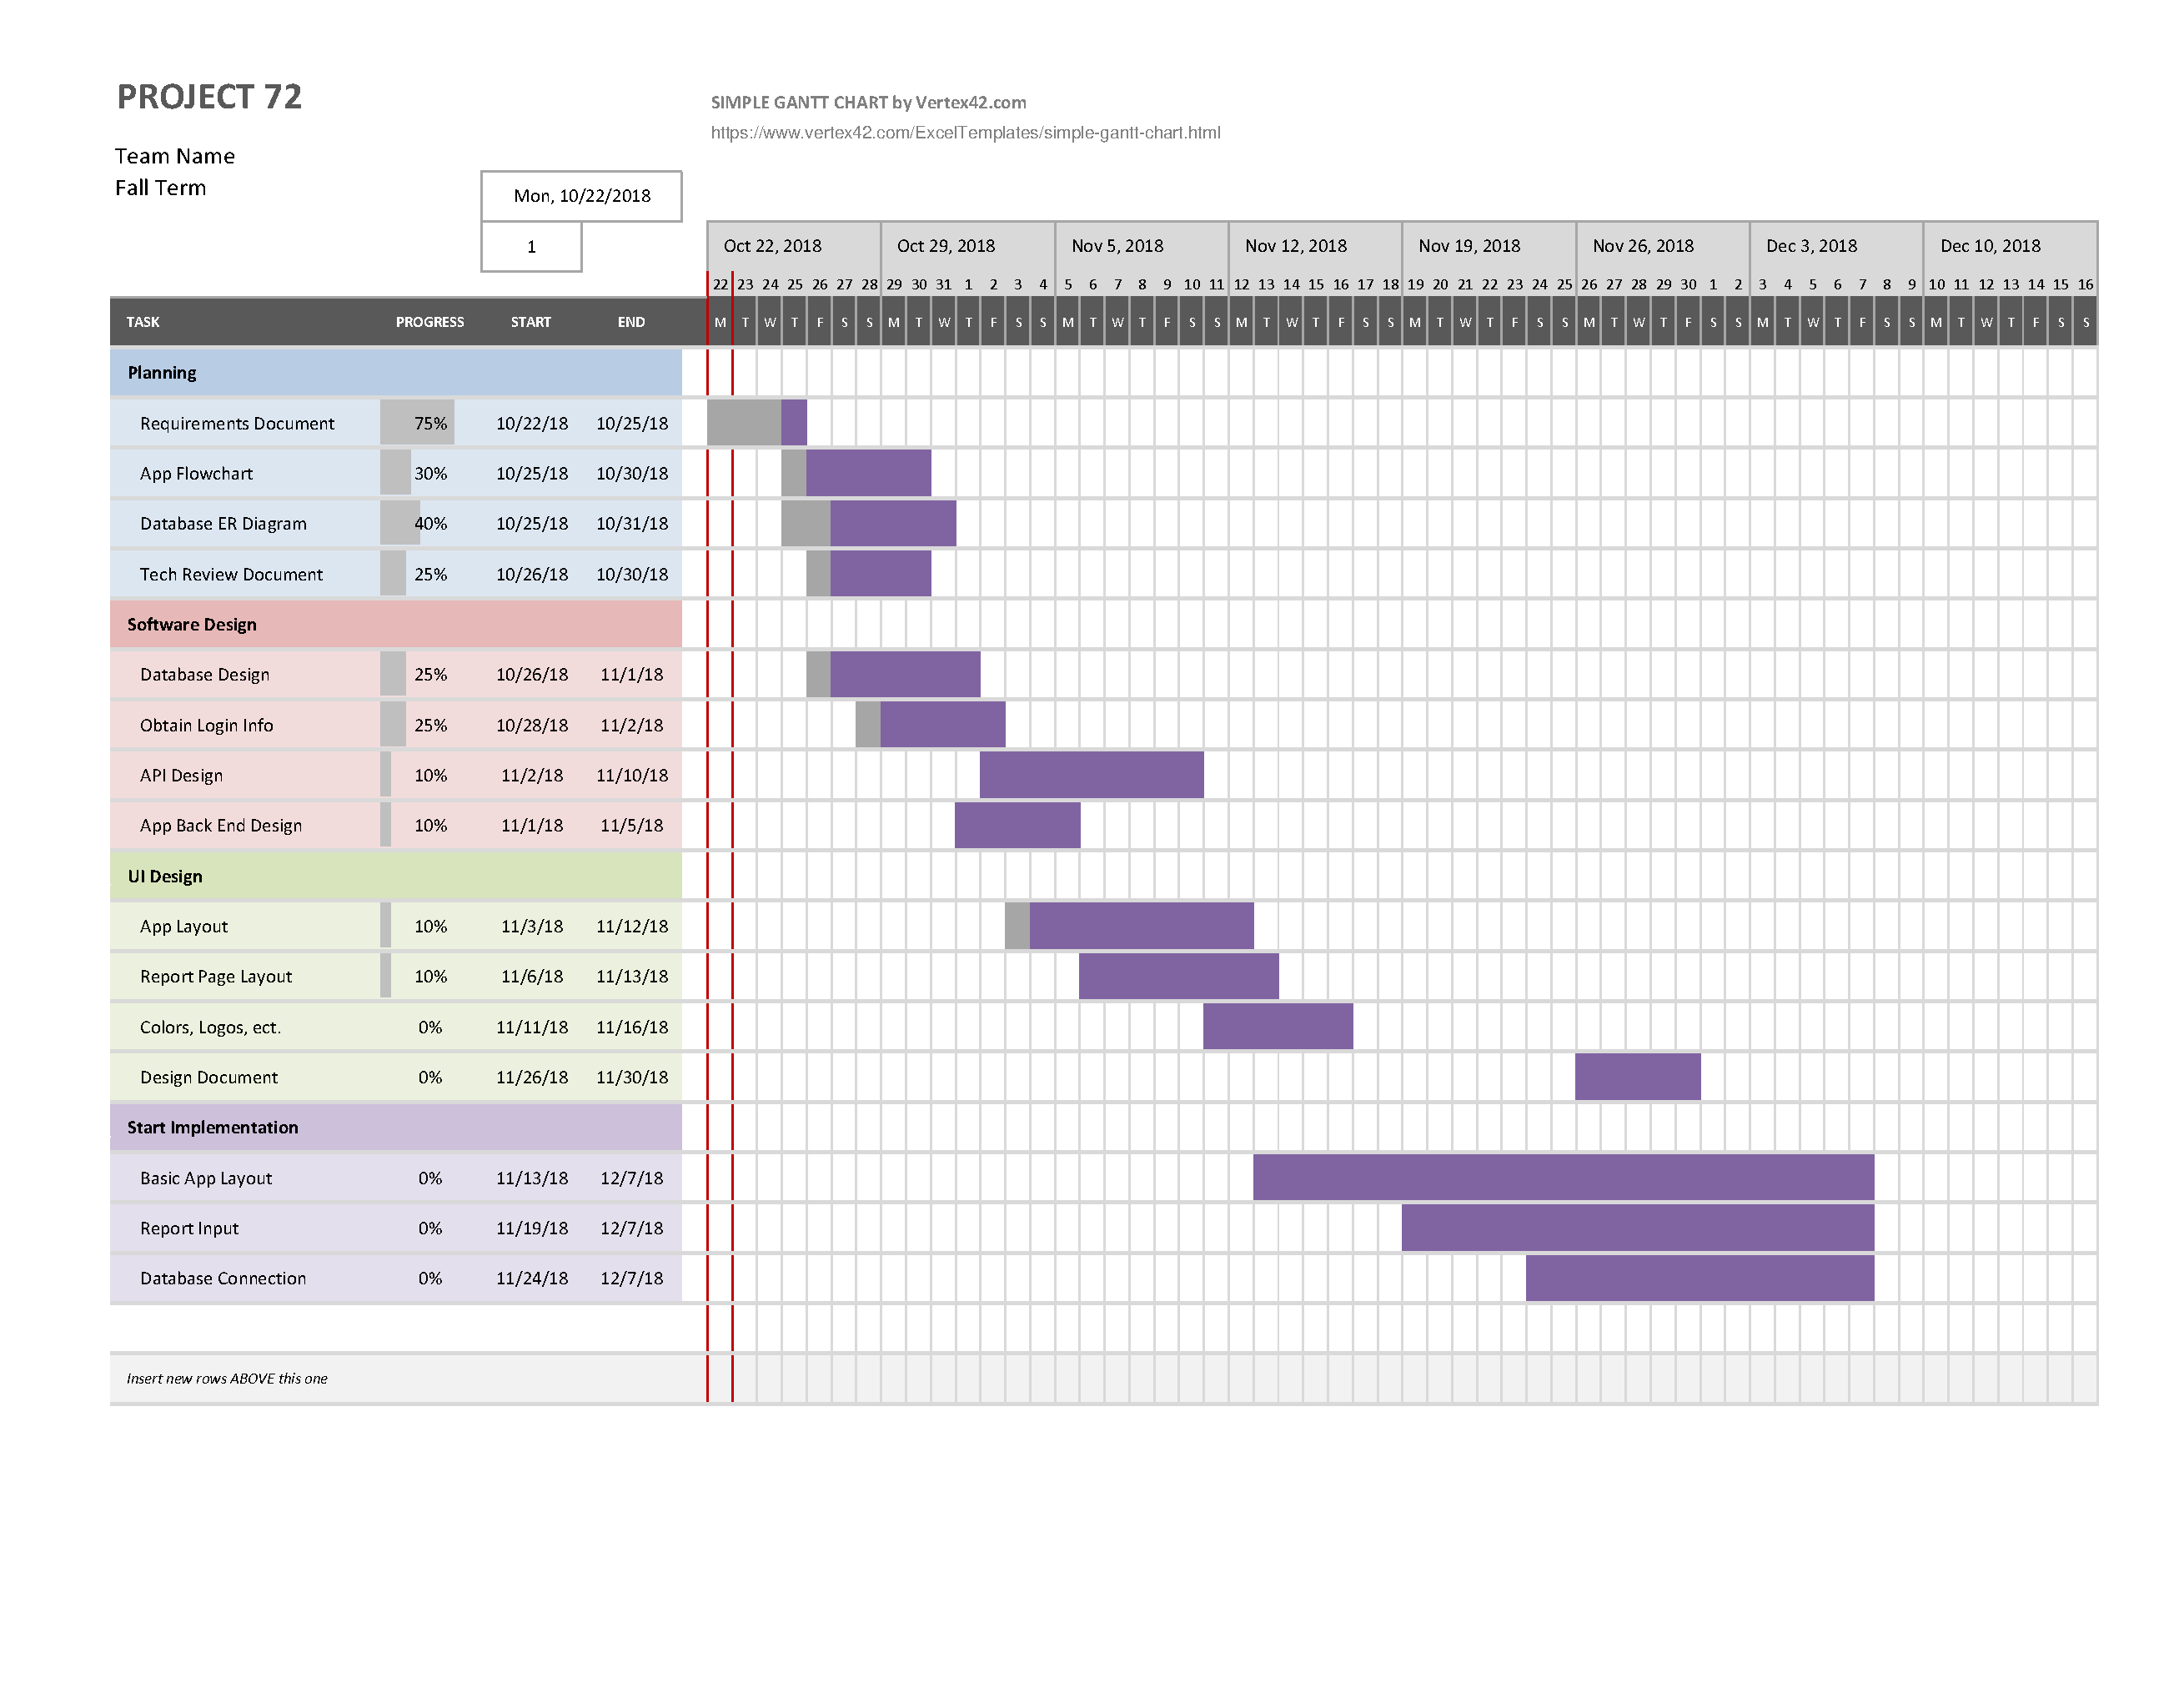
\includepdf[pages=-, angle=90, scale=.8, pagecommand={}]{GanttChart1.pdf}
 
\end{document}








